\documentclass[10pt,a4paper,oneside]{article}
\usepackage{cmap}
\usepackage[T2A]{fontenc}
\usepackage{float}
\usepackage{listings}
\usepackage{csquotes}
\usepackage[utf8]{inputenc}
\usepackage{amsmath}
\usepackage{amsfonts}
\usepackage{amssymb}
\usepackage[english, russian]{babel}%Подключаем русский язык.
\usepackage{graphicx}
\usepackage{geometry} % Меняем поля страницы.
\geometry{left=3cm} %Левое поле.
\geometry{right=2cm} %Правое поле.
\geometry{top=3cm} %Верхнее поле.
\geometry{bottom=2cm} %Нижнее поле.


%Начало документа
\begin{document}

%Создаём титульник.
\begin{titlepage}
\newpage
	%Название ВУЗа и институт.
	\begin{center}
		\Large Санкт-Петербургский Государственный Политехнический Университет\\
		Институт Компьютерных Наук и Технологий\\
	\end{center}
	%Кафедра.
	\begin{center}
		\large\textbf {Высшая школа интеллектуальных систем и суперкомпьютерных технологий}
	\end{center}
	
	%Пропуск места. 
	\vspace{5em}
	%!!!!!!!!!!!!!!!!!!!!!!!!!!!!!!!!!Название работы.
	\begin{center}
		\large{Отчёт по лабораторной работе №9 \\ на тему \\
		\textbf{Дифференцирование и интегрирование} }
	\end{center}
	
	%Делаем пропуск и пишем студента и преподавателя.
	\vspace{25em}
	\begin{flushright}
		\textbf{Работу выполнил\\}Студент группы 3530901/80203 \\ Танашкин В.А.\\
		\textbf{Преподаватель\\}Богач Н.В. 
	\end{flushright}
	
	\vspace{\fill}%В самом низу
	\begin{center}
	Санкт-Петербург, 2021 год	
	\end{center}
\end{titlepage} %Закончили титульный лист.

\section{Настройка проекта}
Перед тем как выполнять задания необходимо настроить проект и сделать все необходимые импорты:

\begin{figure}[H]
        \centering
        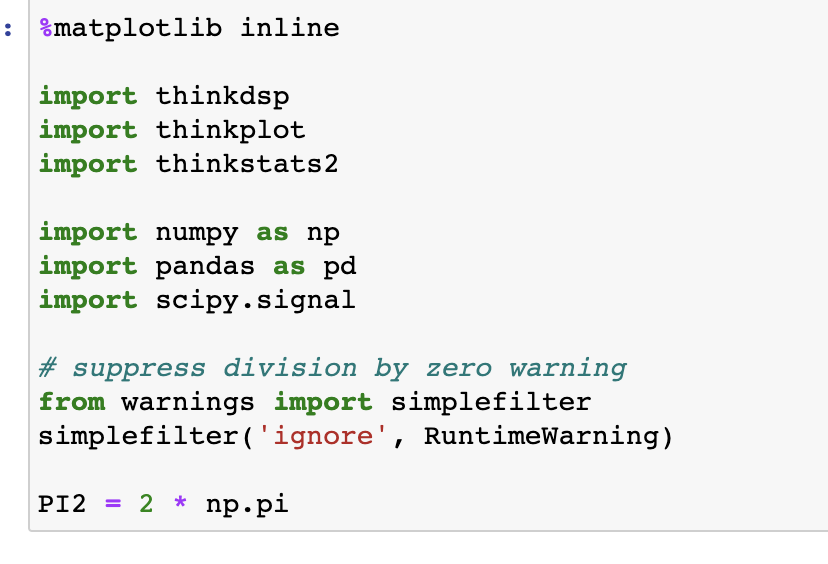
\includegraphics[width=0.75\textwidth]{pics/0.png}
        \caption{2}
        \label{fig:first}
\end{figure}

\section{Упражнение номер №1}

Необходимо создать треугольный сигнал и проверить есть ли различия в воздействии diff и differentiate на этот сигнал? 

Создадим волну треугольного сигнала:

\begin{figure}[H]
        \centering
        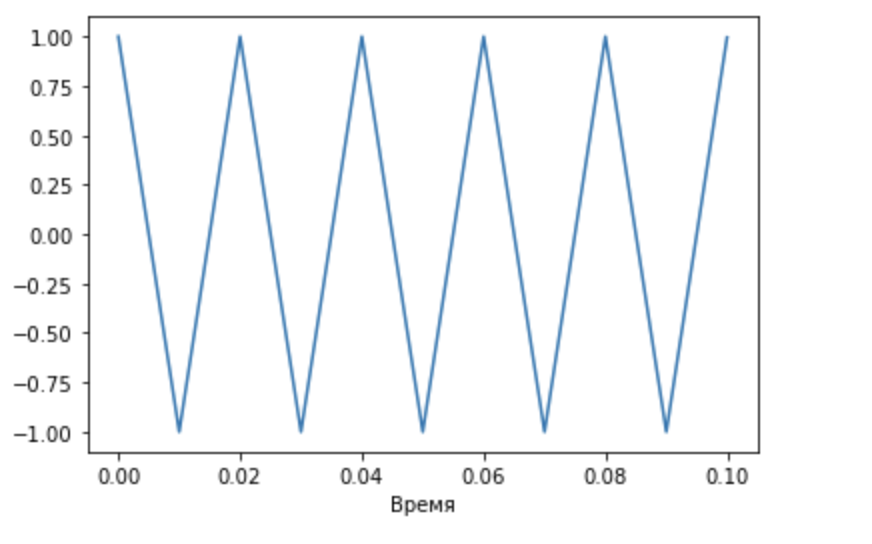
\includegraphics[width=0.75\textwidth]{pics/1.png}
        \caption{2}
        \label{fig:first}
\end{figure}

diff треугольной волны - это прямоугольная волна, что объясняет, почему гармоники в прямоугольной волне уменьшаются как 1/(f) , по сравнению с треугольной волной, которая спадает как 1/(f^2) .

\begin{figure}[H]
        \centering
        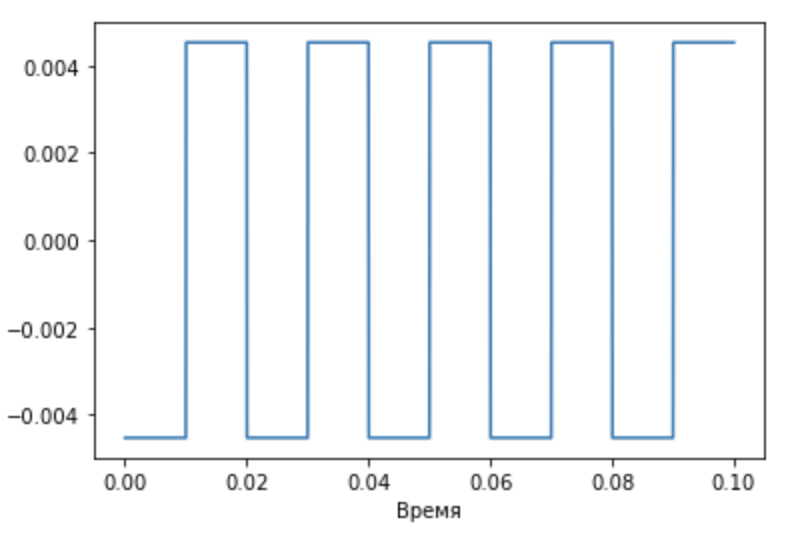
\includegraphics[width=0.75\textwidth]{pics/2.png}
        \caption{2}
        \label{fig:first}
\end{figure}

Когда мы берём спектральную производную, мы получаем "звон" вокруг разрывов.

\begin{figure}[H]
        \centering
        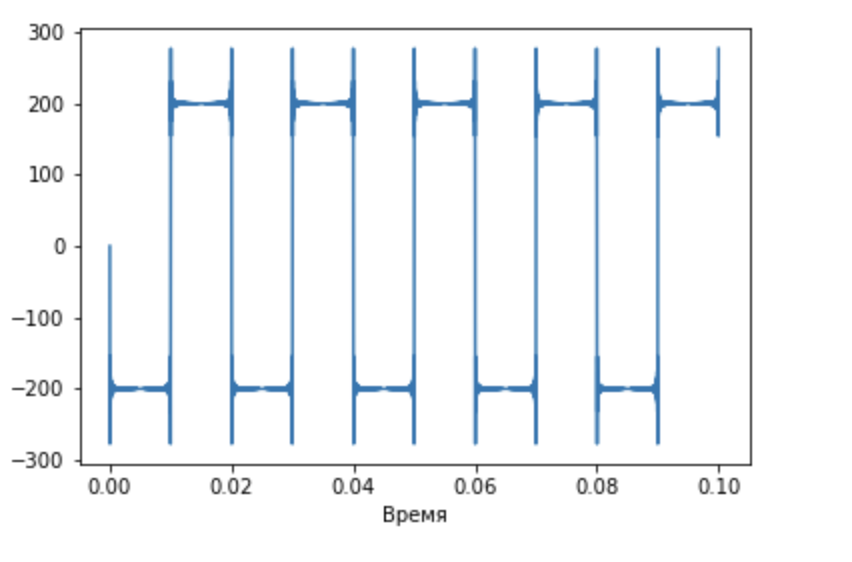
\includegraphics[width=0.75\textwidth]{pics/3.png}
        \caption{2}
        \label{fig:first}
\end{figure}

С математической точки зрения проблема в том, что производная треугольной волны не определена в точках треугольника.

\section{Упражнение номер №2}

Необходимо создать прямоугольный сигнал и проверить есть ли различия в воздействии cumsum и integrate на этот сигнал? 

Создадим волну прямоугольного сигнала:

\begin{figure}[H]
        \centering
        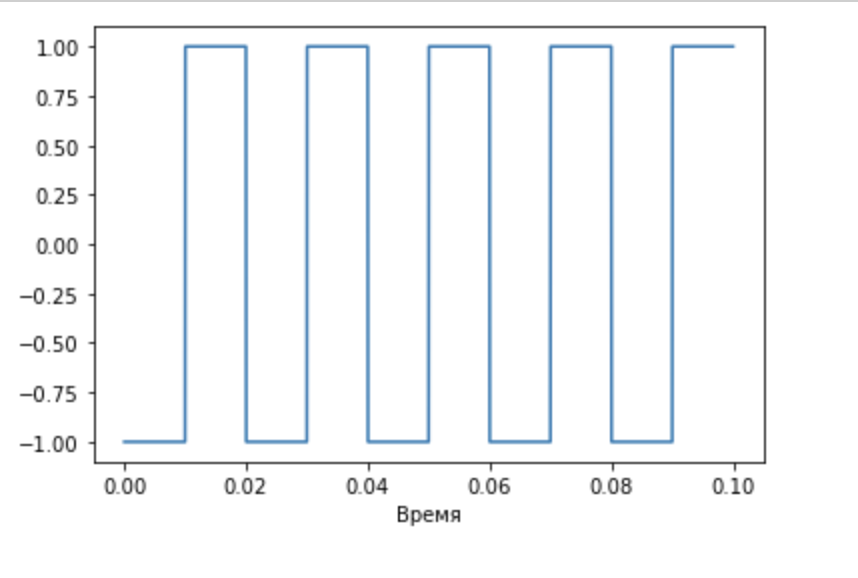
\includegraphics[width=0.75\textwidth]{pics/4.png}
        \caption{2}
        \label{fig:first}
\end{figure}

Совокупная сумма прямоугольной волны - это треугольная волна.

\begin{figure}[H]
        \centering
        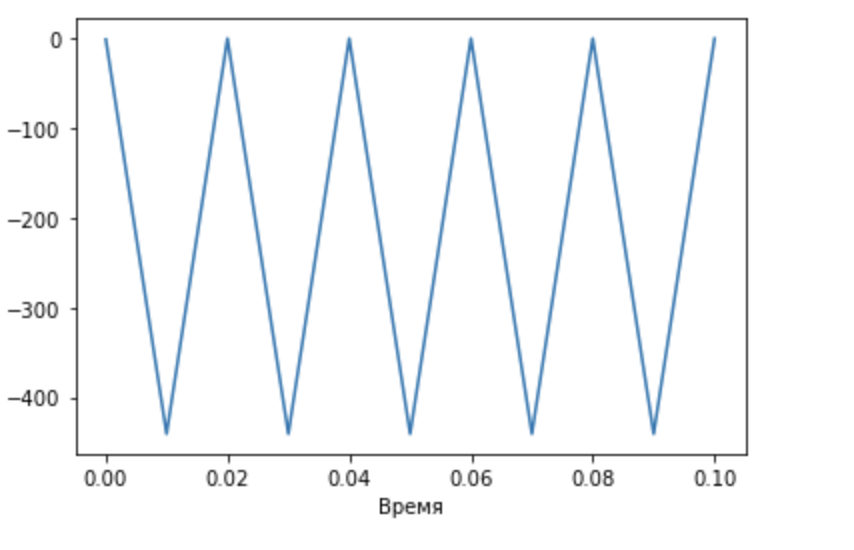
\includegraphics[width=0.75\textwidth]{pics/5.png}
        \caption{2}
        \label{fig:first}
\end{figure}

Спектральный интеграл также представляет собой треугольную волну, несмотря на то что амплитуда сильно отличается.

\begin{figure}[H]
        \centering
        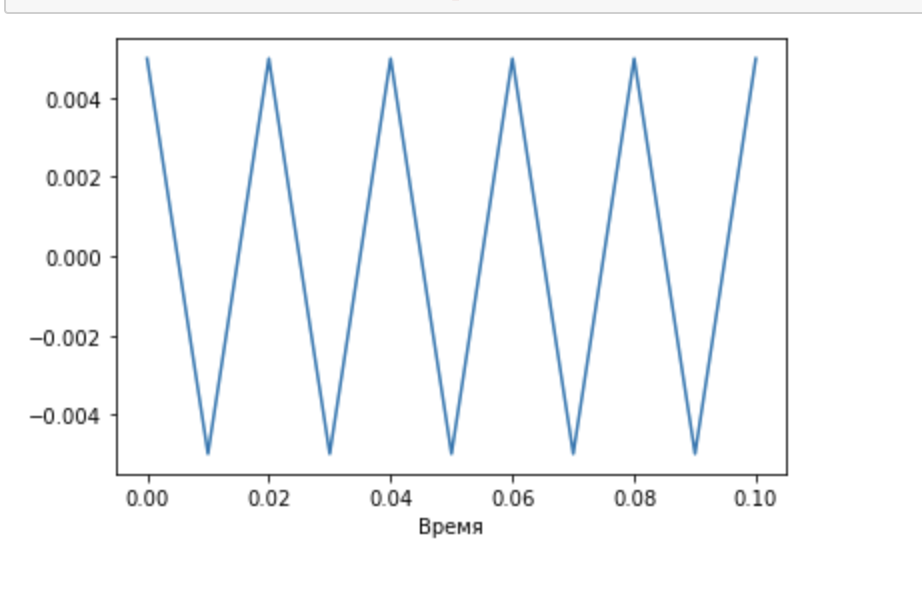
\includegraphics[width=0.75\textwidth]{pics/6.png}
        \caption{2}
        \label{fig:first}
\end{figure}

Если уравновесить и нормализовать две волны, они будут визуально похожи.

\begin{figure}[H]
        \centering
        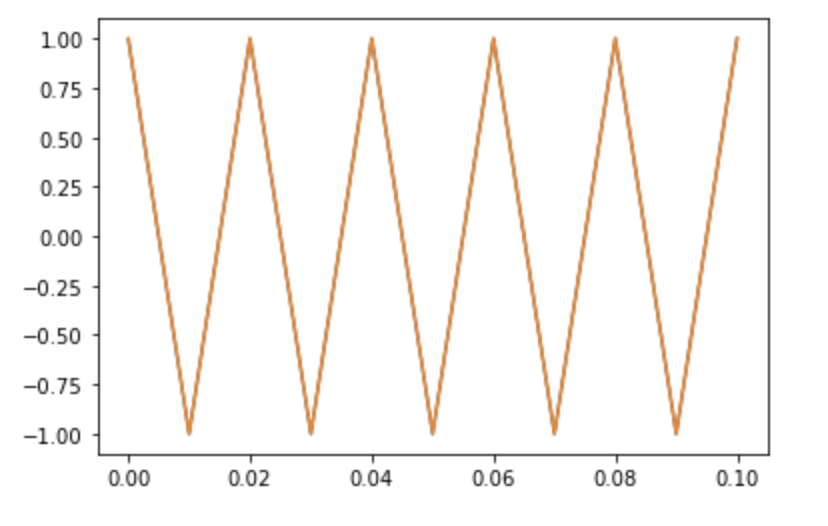
\includegraphics[width=0.75\textwidth]{pics/7.png}
        \caption{2}
        \label{fig:first}
\end{figure}

Численно они также имеют сходство:

\begin{figure}[H]
        \centering
        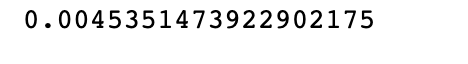
\includegraphics[width=0.75\textwidth]{pics/8.png}
        \caption{2}
        \label{fig:first}
\end{figure}

\section{Упражнение номер №3}

Необходимо создать прямоугольный сигнал. Дважды применить на него integrate. Определить математическую форму сигнала. 

Создадим волну пилообразного сигнала:

\begin{figure}[H]
        \centering
        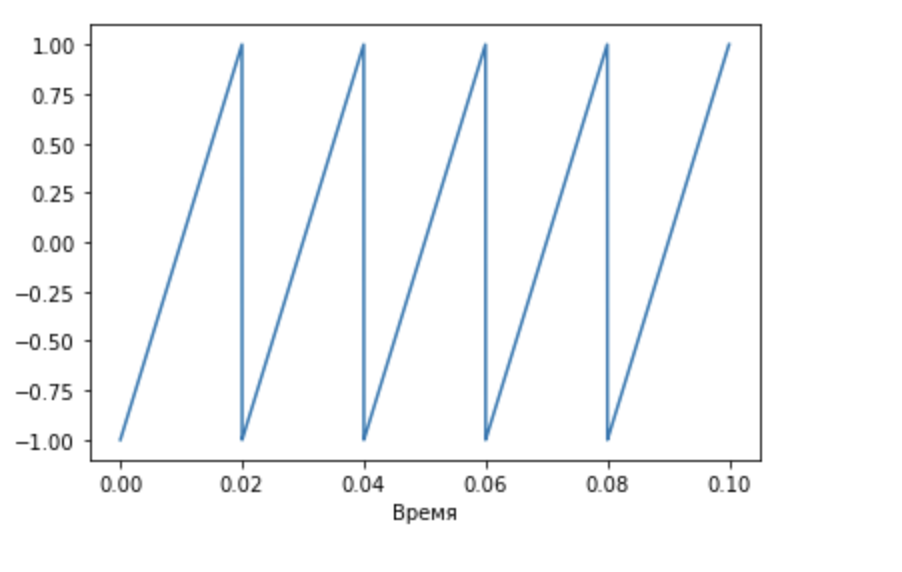
\includegraphics[width=0.75\textwidth]{pics/9.png}
        \caption{2}
        \label{fig:first}
\end{figure}

Первая совокупная сумма зубца пилы - это результат квадратичной функции на графике:

\begin{figure}[H]
        \centering
        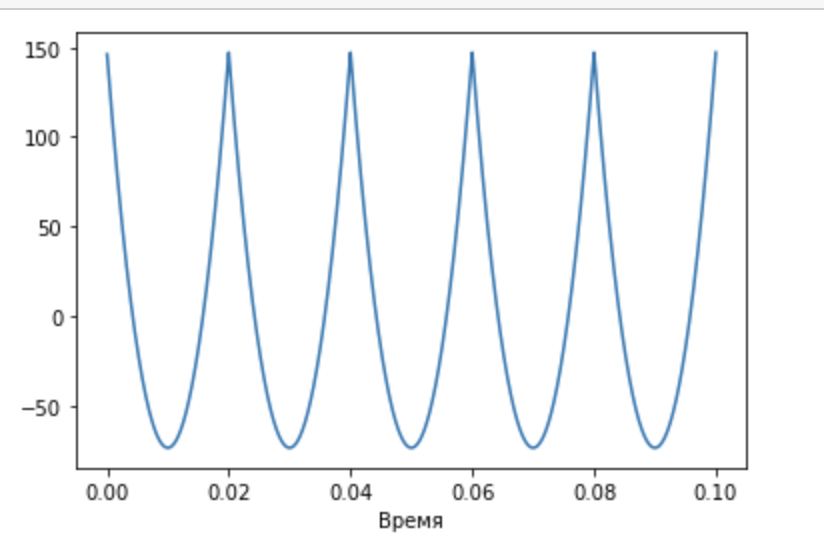
\includegraphics[width=0.75\textwidth]{pics/10.png}
        \caption{2}
        \label{fig:first}
\end{figure}

Вторая совокупная сумма - это кубическая кривая:

\begin{figure}[H]
        \centering
        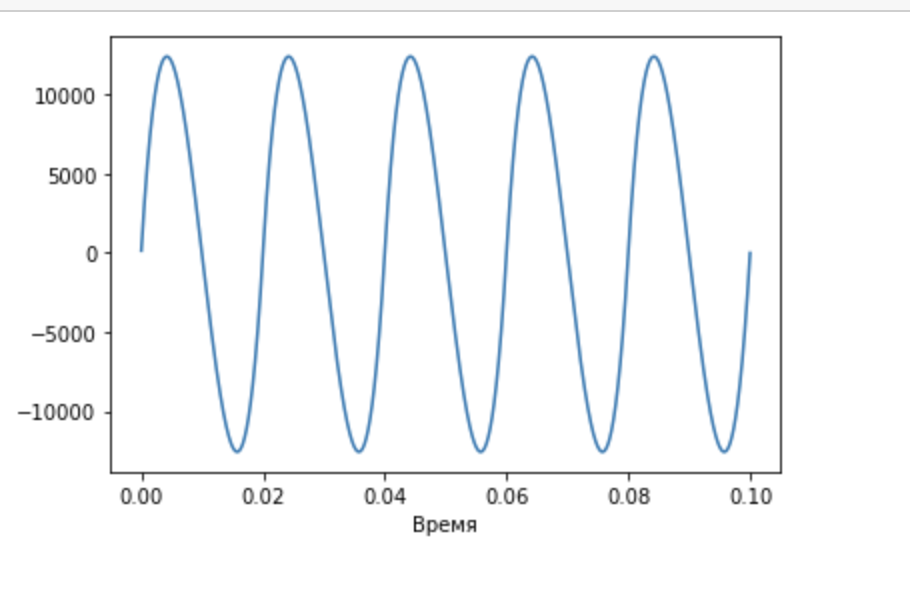
\includegraphics[width=0.75\textwidth]{pics/11.png}
        \caption{2}
        \label{fig:first}
\end{figure}

Двойное интегрирование также дает кубическую кривую.

\begin{figure}[H]
        \centering
        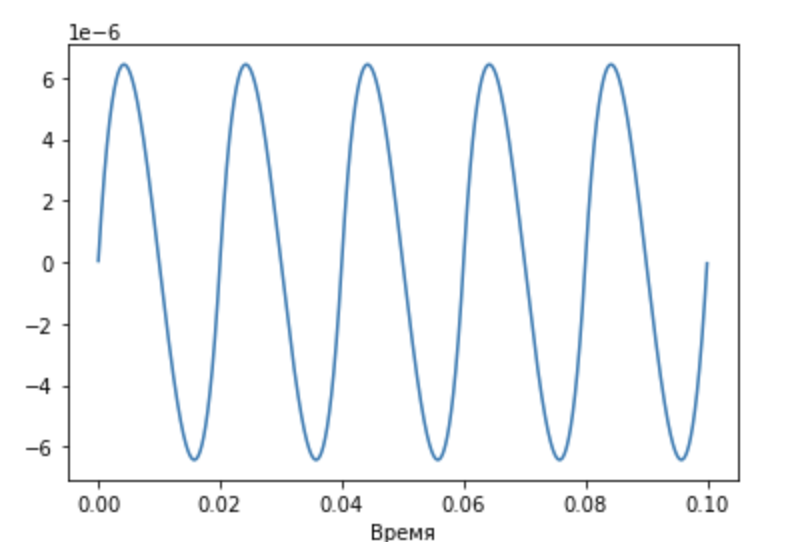
\includegraphics[width=0.75\textwidth]{pics/12.png}
        \caption{2}
        \label{fig:first}
\end{figure}

На этом этапе результат всё больше и больше напоминает синусоиду. Причина в том, что интеграция действует как фильтр нижних частот. На данный момент мы отфильтровали почти все, кроме основного, как показано в спектре ниже:

\begin{figure}[H]
        \centering
        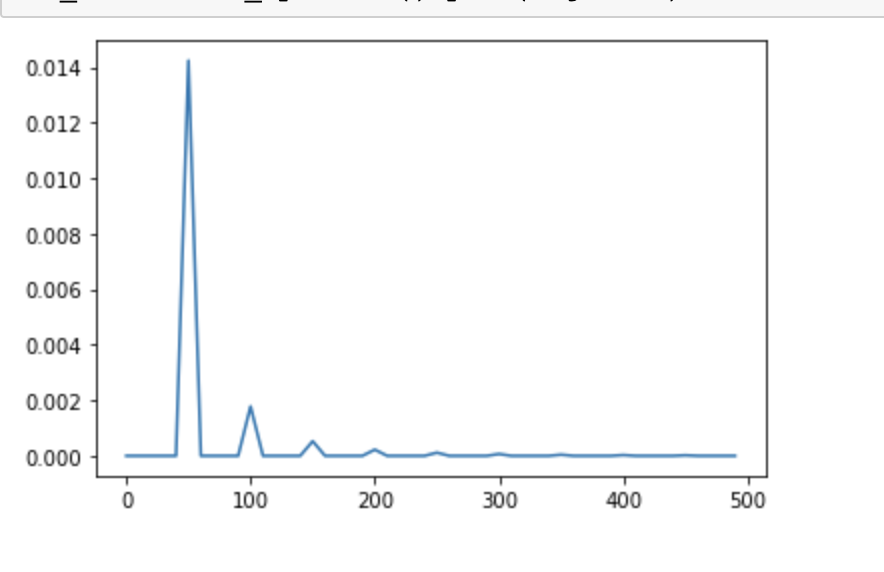
\includegraphics[width=0.75\textwidth]{pics/13.png}
        \caption{2}
        \label{fig:first}
\end{figure}

\section{Упражнение номер №4}

Необходимо создать CubicSignal, вычислить вторую разность. Распечать фильтры соотвествующие второй разнице и второй производной и сравнить их.

Создадим волну кубического сигнала:

\begin{figure}[H]
        \centering
        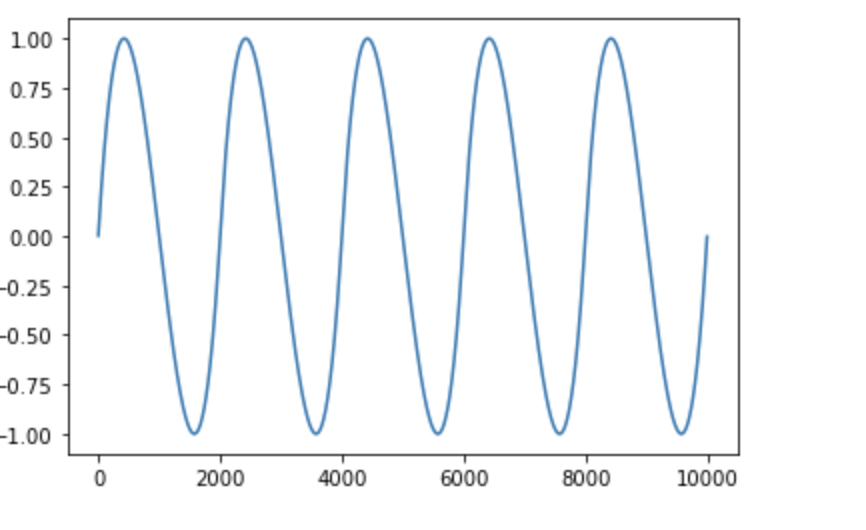
\includegraphics[width=0.75\textwidth]{pics/14.png}
        \caption{2}
        \label{fig:first}
\end{figure}

Первая разность - парабола, вторая - пилообразная волна:

\begin{figure}[H]
        \centering
        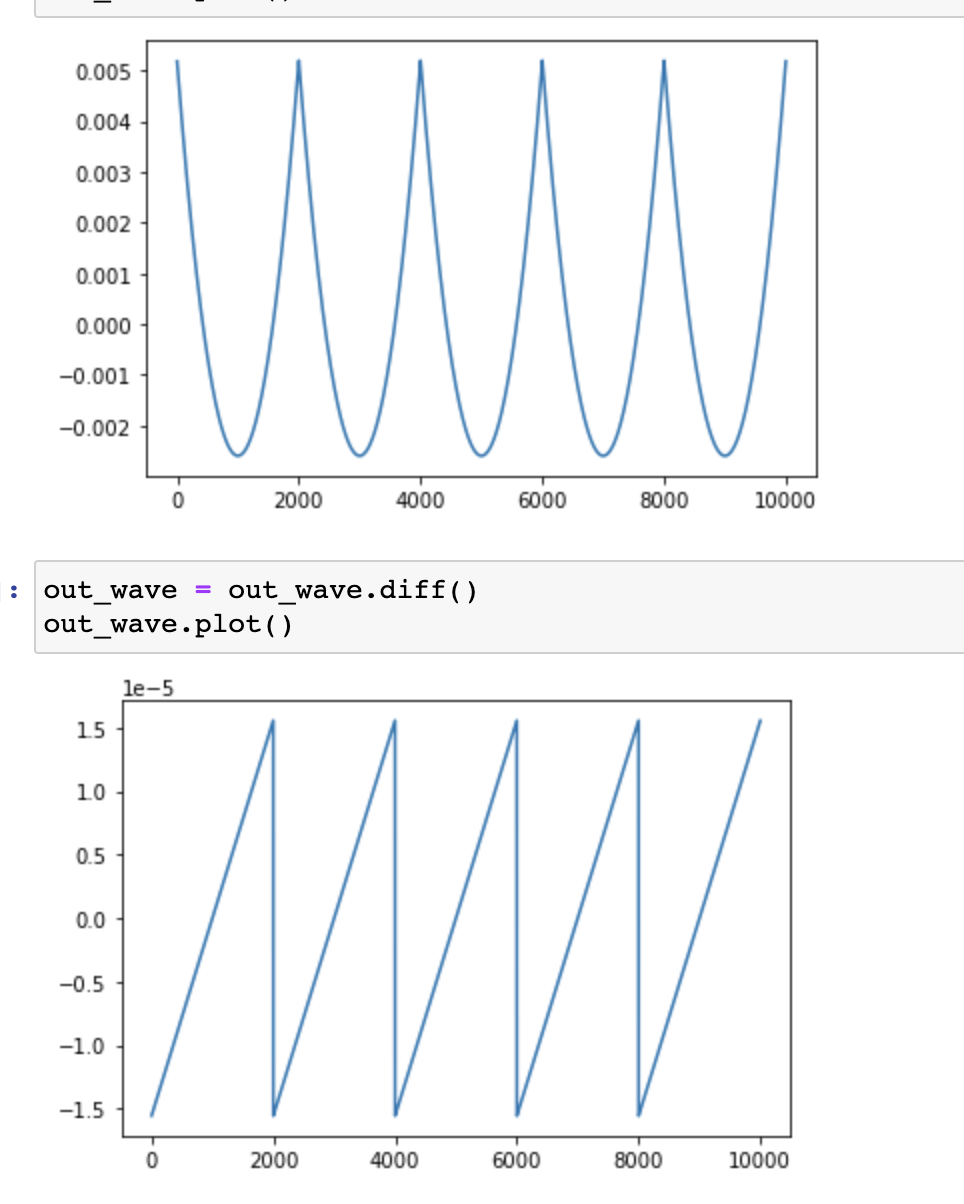
\includegraphics[width=0.75\textwidth]{pics/15.png}
        \caption{2}
        \label{fig:first}
\end{figure}

Когда мы дифференцируем дважды, получаем пилообразную форму с некоторым звоном. Проблема в том, что производная параболического сигнала в точках не определена.

\begin{figure}[H]
        \centering
        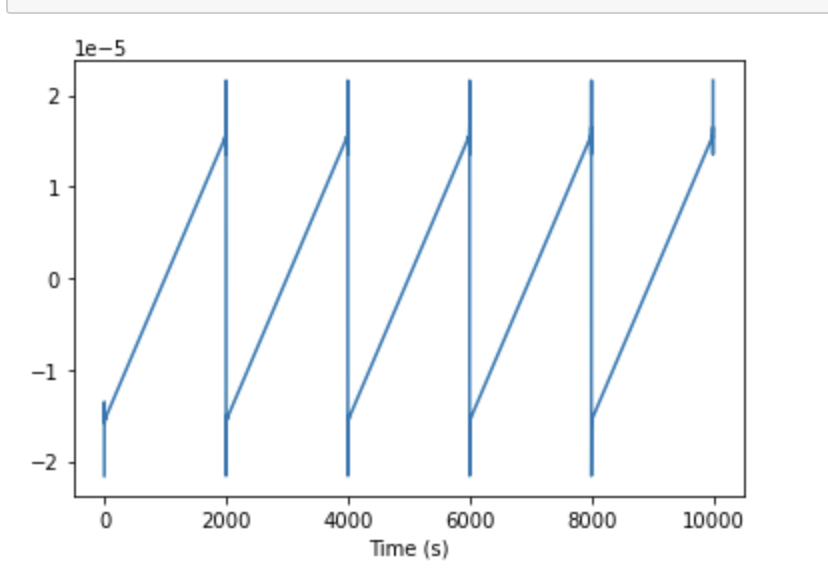
\includegraphics[width=0.75\textwidth]{pics/16.png}
        \caption{2}
        \label{fig:first}
\end{figure}

Окно второй разности -1, 2, -1. Вычисляя DFT окна, мы можем найти соответствующий фильтр.

\begin{figure}[H]
        \centering
        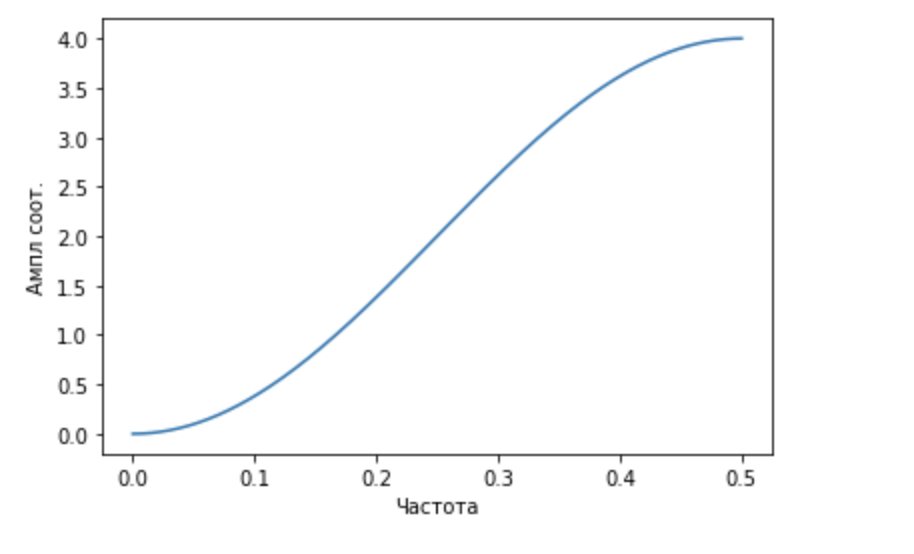
\includegraphics[width=0.75\textwidth]{pics/17.png}
        \caption{2}
        \label{fig:first}
\end{figure}

А для второй производной мы можем найти соответствующий фильтр, вычислив фильтр первой производной и возведя его в квадрат.

\begin{figure}[H]
        \centering
        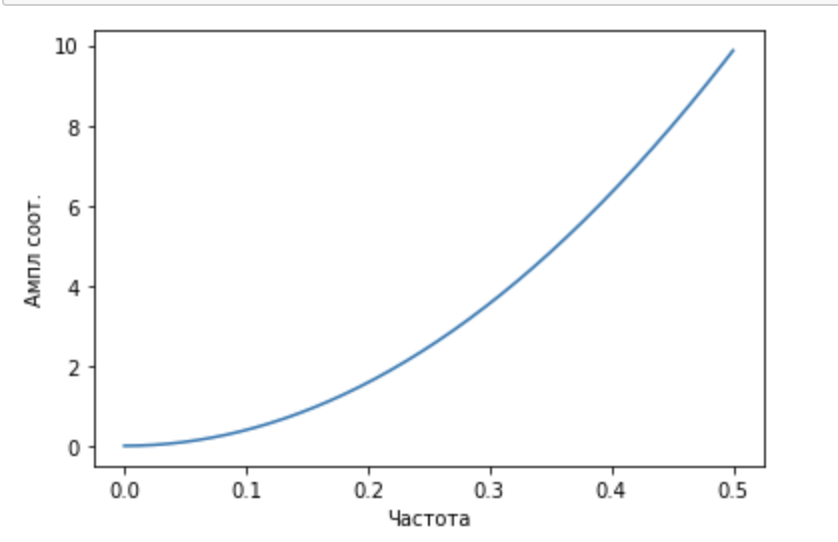
\includegraphics[width=0.75\textwidth]{pics/18.png}
        \caption{2}
        \label{fig:first}
\end{figure}

Сравним полученные функции в одной системе:

\begin{figure}[H]
        \centering
        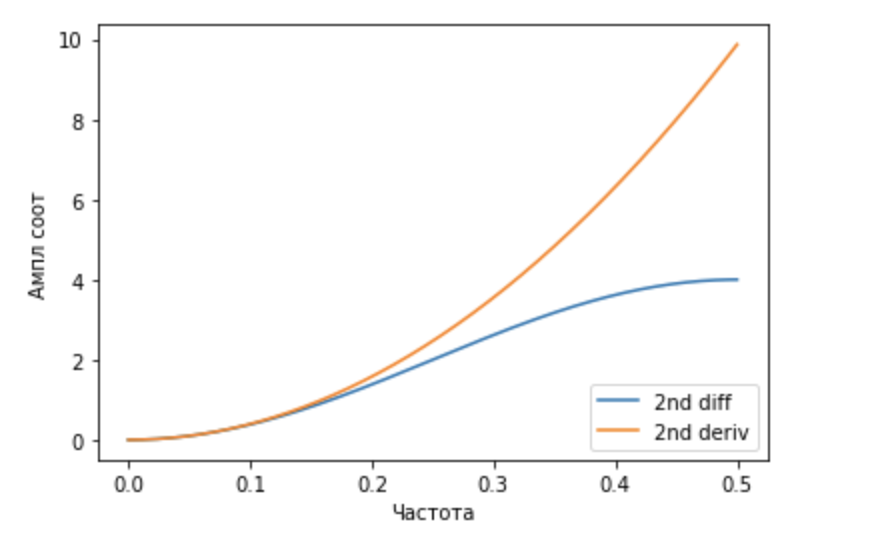
\includegraphics[width=0.75\textwidth]{pics/19.png}
        \caption{2}
        \label{fig:first}
\end{figure}

Оба являются фильтрами высоких частот, которые усиливают компоненты самых высоких частот. Вторая производная параболическая, поэтому она сильнее всего усиливает самые высокие частоты. Вторая разница - хорошее приближение второй производной только на самых низких частотах, затем она существенно отклоняется.

\end{document}
